\section{Phép đếm}
\subsection{Kiến thức cần nhớ}
%\subsection{Bài tập mẫu}
\Opensolutionfile{ans}[ans/ANS-DANG-47]
\begin{khung}
	\begin{vd}[Đề minh họa BGD 2022-2023]
		Có bao nhiêu cặp số nguyên $(x;y)$ thỏa mãn
\begin{align*}
\log_3\left(x^2+y^2+x\right)+\log_2\left(x^2+y^2\right)\le \log_3x+\log_2\left(x^2+y^2+24x\right)?
\end{align*}
		\loigiai{
		Điều kiện $x>0$\\
Ta có: $\log_3\left(x^2+y^2+x\right)+\log_2\left(x^2+y^2\right)\le \log_3x+\log_2\left(x^2+y^2+24x\right)$
\begin{align*}
&\Leftrightarrow \log_3\left(x^2+y^2+x\right)-\log_3x\le \log_{2}\left(x^2+y^2+24x\right)-\log_{2}\left(x^2+y^2\right)\\ 
& \log_3\left(\dfrac{x^2+y^2+x}{x}\right)\le \log_2\left(\dfrac{x^2+y^2+24x}{x^2+y^2}\right)\Leftrightarrow \log_3\left(1+\dfrac{x^2+y^2}{x}\right)\le \log_2\left(1+\dfrac{24x}{x^2+y^2}\right)\\
&\Leftrightarrow \log_3\left(\dfrac{x^2+y^2}{x}+1\right)-\log_2\left(1+\dfrac{24x}{x^2+y^2}\right)\le 0. 
\end{align*}
Đặt: $t=\dfrac{x^2+y^2}{x},(t>0)$, bất phương trình trở thành: $\log_3(1+t)-\log_2\left(1+\dfrac{24}{t}\right)\le 0$ \hfill (1).\\
Xét hàm số $f(t)=\log_3(1+t)-\log_2\left(1+\dfrac{24}{t}\right)$ có $f'(t)=\dfrac{1}{(1+t)\ln 3}+\dfrac{24}{\left(t^2+24t\right)\ln 2}>0,\forall t>0$.\\
Suy ra hàm số đồng biến trên $\left(0;+\infty\right)$.\\
Ta có $f(8)=\log_3(1+8)-\log_2\left(1+\dfrac{24}{8}\right)=0$.\\
Từ đó suy ra: $(1)\Leftrightarrow f(t)\le f(8)\Leftrightarrow \dfrac{x^2+y^2}{x}\le 8\Leftrightarrow (x-4)^2+y^2\le 16$.\\
Đếm các cặp giá trị nguyên của $(x;y)$.\\
Ta có: $\left(x-4\right)^2\le 16\Leftrightarrow 0\le x\le 8$, mà $x>0$ nên $0<x\le 8$.\\
Với $x=1,x=7\Rightarrow y=\left\{\pm 2;\pm 1;0\right\}$ nên có 10 cặp.\\
Với $x=2,x=6\Rightarrow y=\left\{\pm 3;\pm 2;\pm 1;0\right\}$ nên có 14 cặp.\\
Với $x=3,x=5\Rightarrow y=\left\{\pm 3;\pm 2;\pm 1;0\right\}$ nên có 14 cặp.\\
Với $x=4,x=6\Rightarrow y=\left\{\pm 4;\pm 3;\pm 2;\pm 1;0\right\}$ nên có 9 cặp.\\
Với $x=8\Rightarrow y=0$ có 1 cặp.\\
Vậy có 48 cặp giá trị nguyên $(x;y)$ thỏa mãn đề bài.
	}
	\end{vd}
\end{khung}
\subsection{Bài tập tương tự và phát triển}
\begin{ex}%[2D2G5-5]
	Cho hàm số $f(x)=\log_2\left(x+\sqrt{x^2+1}\right)$. Có bao nhiêu cặp số nguyên $(a; b)$ thỏa mãn $f\left(2^{a^2-ab+b}-\dfrac{1}{4}\right)+f\left(\left(a^2-ab+b+2\right)2^{b-2-ab}\right)=0$. 
	\choice
	{\True $4$}
	{$3$}
	{$2$}
	{$5$}
	\loigiai{
		Ta có hàm $f(x)$ xác định, liên tục trên $\mathbb{R}$ và $f'(x)=\dfrac{1}{\ln 2\cdot\sqrt{x^2+1}}>0,\forall x\in\mathbb{R}$ \\
		$ \Rightarrow f(x) $ đồng biến trên $\mathbb{R}$.\\
		Mặt khác $f(-x)=\log_2\left(-x+\sqrt{x^2+1}\right)=-\log_2\left(x+\sqrt{x^2+1}\right)=-f(x),\forall x\in\mathbb{R}$;\\
		suy ra $f(x)$ là hàm số lẻ trên $\mathbb{R}$.\\
		Ta có:
		\begin{align*}
&f\left(2^{a^2-ab+b}-\dfrac{1}{4}\right)+f\left(\left(a^2-ab+b+2\right)2^{b-2-ab}\right)=0\\&\Leftrightarrow f\left(2^{a^2-ab+b}-\dfrac{1}{4}\right)=-f\left(\left(a^2-ab+b+2\right)2^{b-2-ab}\right)\\&\Leftrightarrow f\left(2^{a^2-ab+b}-\dfrac{1}{4}\right)=f\left(\left(-a^2+ab-b-2\right)2^{b-2-ab}\right)\\&\Leftrightarrow 2^{a^2-ab+b}-\dfrac{1}{4}=\left(-a^2+ab-b-2\right)2^{b-2-ab}\\&\Leftrightarrow 2^{a^2+2}+a^2+2=2^{ab-b}+ab-b. \tag{1}
\end{align*}
		Xét hàm số $g(t)=2^t+t, t\in\mathbb{R};$ có $g'(t)=2^t\cdot\ln 2+1>0,\forall t\in\mathbb{R}\Rightarrow g(t)$ đồng biến trên $\mathbb{R}$.\\
		$(1)\Leftrightarrow g\left(a^2+2\right)=g(ab-b)\Leftrightarrow a^2+2=ab-b\Leftrightarrow b(a-1)=a^2+2(2)$.\\
		Nhận xét $a=1$ không thỏa $(2)$. Với $a\neq 1$ ta có $b=\dfrac{a^2+2}{a-1}=a+1+\dfrac{3}{a-1}$.\\
		Vì $a, b$ nguyên nên $\hoac{&a-1=-3\\&a-1=-1\\&a-1=1\\&a-1=3}\Leftrightarrow\hoac{&a=-2\Rightarrow b=-2\\&a=0\Rightarrow b=-2\\&a=2\Rightarrow b=6\\&a=4\Rightarrow b=6.}$ \\
		Vậy có 4 cặp số nguyên $(a;b)$ là $(-2;-2);(0;-2);(2;6);(4;6)$.}
\end{ex}

\begin{ex}%[2D2G5-5]
	Có bao nhiêu bộ hai số nguyên $(x;y)$ thỏa $1\leq x^2+x\leq 2020$ và 
	$$\log x+\log (x+1) +x^2+x =y +10^y$$ 
	\choice
	{2}
	{\True 0}
	{8}
	{4}
	\loigiai{
		Điều kiện: $x>0$.\\
		Ta có: 
\begin{align*}
&\log x+\log (x+1)+x^2+x=y+10^y\\
& \Leftrightarrow\log [x(x+1)]+x^2+x=y+10^y \Leftrightarrow\log (x^2+x)+x^2+x=\log (10^y)+10^y 
\end{align*}
		Xét hàm số: $f(t)=\log t+t$ với $t>0$.\\
		$f'(t)=\dfrac{1}{t\ln 10}+1>0$, $\forall t>0$.\\
		Hàm số đồng biến trên khoảng $(0;+\infty)$ 
		$ \Rightarrow x^2+x=10^y $.\\
		Vì $1\leq x^2+x\leq 2020$ nên $1\leq 10^y\leq 2020\Leftrightarrow 0\leq y\leq\log 2020\approx 3,305$.\\
		Mà $y$ chỉ nhận giá trị nguyên nên $y\in\{0;1;2;3\}$.
\begin{align*}
&+) y=0\Rightarrow x=\dfrac{-1+\sqrt{5}}{2} \text{(loại)}.\\
&+) y=1\Rightarrow x=\dfrac{-1+\sqrt{41}}{2} \text{(loại)}.\\
&+) y=2\Rightarrow x=\dfrac{-1+\sqrt{401}}{2} \text{(loại)}.\\
&+) y=3\Rightarrow x=\dfrac{-1+\sqrt{4001}}{2} \text{(loại)}.
\end{align*}
		Vậy không có bộ hai số nguyên $(x;y)$ thỏa mãn yêu cầu bài toán.}
\end{ex}
\begin{ex}%[2D2G5-5]
	Cho $a>0, b>0$ thỏa mãn $\log_{10a+3b+1}\left(25a^2+b^2+1\right)+\log_{10ab+1}(10a+3b+1)=2$. Giá trị biểu thức $a+2b$ bằng
	\choice
	{$22$}
	{$6$}
	{\True $\dfrac{11}{2}$}
	{$\dfrac{5}{2}$}
	\loigiai{
		Với $a>0,b>0$ ta có $25a^2+b^2+1\geq 10ab+1$.\\
 Dấu “=” xảy ra khi và chỉ khi $b=5a$.\\
		Suy ra $\log_{10a+3b+1}\left(25a^2+b^2+1\right)\geq\log_{10a+3b+1}(10ab+1)$\\
 Dấu “=” xảy ra khi và chỉ khi $b=5a$.\\
		Mặt khác, ta lại có với $a>0,b>0$ thì $\log_{10a+3b+1}(10ab+1)>0,\log_{10ab+1}(10a+3b+1)>0$.\\
		Do đó:
	\begin{align*}
\log_{10a+3b+1}\left(25a^2+b^2+1\right)+\log_{10ab+1}(10a+3b+1)&\geq\log_{10a+3b+1}(10ab+1)+\log_{10ab+1}(10a+3b+1)\\
& \geq 2\sqrt{\log_{10a+3b+1}(10ab+1)\cdot\log_{10ab+1}(10a+3b+1)}=2
\end{align*}	
		Dấu “=” xảy ra khi và chỉ khi
		\begin{eqnarray*}
		&&\heva{&b=5a\\&\log_{10a+3b+1}(10ab+1)=\log_{10ab+1}(10a+3b+1)}\\
		&\Leftrightarrow&\heva{&b=5a\\&10a+3b+1=10ab+1}\\
		&\Leftrightarrow&\heva{&b=\dfrac{5}{2}\\&a=\dfrac{1}{2}}\Rightarrow a+2b=\dfrac{11}{2}.
		\end{eqnarray*} }
\end{ex}
\begin{ex}%[2D2G5-5]
	Hỏi có bao nhiêu số nguyên $y$ sao cho mỗi giá trị của $y$ có không quá $2021$ số nguyên $x$ thỏa mãn $\log_2\left(x+y^2+1\right)-3^{y^2+y-3x}<0$?
	\choice
	{$109$}
	{$108$}
	{\True $110$}
	{$111$}
	\loigiai{
		Xét hàm số $f(t)=\log_2t-3^{-3t+2y^2+y+3}$ trên $(0;+\infty)$.\\
		$f'(t)=\dfrac{1}{t\ln 2}+3\cdot 3^{-3t+2y^2+y+3}\cdot\ln 3>0\forall t\in(0;+\infty)$ \\
		$ \Rightarrow $ Hàm số $f(t)$ đồng biến trên $(0;+\infty)$.\\
		Do có không quá $2021$ số nguyên $x$ nên có không quá $2021$ số nguyên của $t$ \\
		$ \Rightarrow t $ nguyên thuộc $[1; 2021]$ thì $f(t)<0$ và $f(2022)>0$ \\
		$ \Leftrightarrow\log_22022-3^{2y^2+y-6060}\geq 0\Leftrightarrow 2y^2+y-6060-\log_3\left(\log_22022\right)\leq 0 $.\\
		Do $y$ nguyên nên $y\in\left\{-55;-54;\ldots; 54\right\}$.\\
		Vậy có $110$ số nguyên $y$ thỏa mãn yêu cầu bài toán.}
\end{ex}
\begin{ex}%[2D2G5-5]
	Cho các số thực $x,y$ thỏa mãn $2x-y=\mathrm{e}^x\left(2-\mathrm{e}^x\right)+\ln \left(2\mathrm{e}^x+y\right)$. Tìm giá trị nhỏ nhất của biểu thức $P=x^2+y^2+20y$. 
	\choice
	{$0$}
	{$-21$}
	{$-100$}
	{\True $-19$}
	\loigiai{
		Điều kiện $2\mathrm{e}^x+y>0$ (*).\\
		Ta có
	\begin{align*}
&2x-y=\mathrm{e}^x\left(2-\mathrm{e}^x\right)+\ln \left(2\mathrm{e}^x+y\right)\\
& \Leftrightarrow\mathrm{e}^{2x}+2x=\ln \left(2\mathrm{e}^x+y\right)+2\mathrm{e}^x+y\tag{1}
\end{align*}	
		Đặt $\mathrm{e}^{2x}=u\Rightarrow 2x=\ln u$, phương trình (1) viết lại thành:
\begin{align*}
&\ln u+u=\ln \left(2\mathrm{e}^x+y\right)+2\mathrm{e}^x+y \tag{2}
\end{align*}
		Xét hàm số $f(t)=\ln t+t, t>0$ có $f'(t)=\dfrac{1}{t}+1>0,\forall t>0$ nên $f(t)$ đồng biến trên $(0;+\infty)$.\\
		Do đó $(2)\Leftrightarrow u=2\mathrm{e}^x+y$, ta thu được phương trình:
\begin{align*}
&\mathrm{e}^{2x}=2\mathrm{e}^x+y\Leftrightarrow y=\mathrm{e}^{2x}-2\mathrm{e}^x\Rightarrow y+1=\left(\mathrm{e}^x-1\right)^2\geq 0\Rightarrow y\geq-1
\end{align*}
		Khi đó $P=x^2+y^2+20y=x^2+(y+1)^2+18y-1\geq 0+0-18-1=-19$.\\
		Đẳng thức xảy ra khi $x=0; y=-1$ thỏa điều kiện (*).}
\end{ex}
\begin{ex}%[2D2G5-5]
	Cho $x$, $y$ là các số thực thỏa mãn $\log_3(x+y)=\log_4\left(x^2+y^2\right)$. Tập giá trị của biểu thức $P=x^3+y^3$ có chứa bao nhiêu giá trị nguyên?
	\choice
	{$9$}
	{Vô số}
	{\True $4$}
	{$5$}
	\loigiai{
		+Điều kiện $x+y>0$; $x^2+y^2\neq 0$.\\
		Ta đặt: $\log_3(x+y)=\log_4\left(x^2+y^2\right)=t$.\\
		Ta có $\heva{&x+y=3^t\\&x^2+y^2=4^t}(1)$.\\
		Vì $(x+y)^2\leq 2\left(x^2+y^2\right)\Rightarrow(3^t)^2\leq 2\cdot 4^t\Rightarrow t\leq\log_{\tfrac{9}{4}}^2\approx 0,85$.\\
		+ Ta có $x^2+y^2=(x+y)^2-2xy\Rightarrow xy=\dfrac{9^t-4^t}{2}$.\\
		+ Khi đó, $P=x^3+y^3=(x+y)^3-3xy(x+y) =27^t-3\cdot 3^t\cdot\dfrac{9^t-4^t}{2} =-\dfrac{1}{2}\cdot 27^t+\dfrac{3}{2}\cdot 12^t=f(t)$.\\
		+ Xét $f(t)=-\dfrac{1}{2}\cdot 27^t+\dfrac{3}{2}\cdot 12^t$ với $t\leq\log_{\tfrac{9}{4}}^2$, có $f'(t)=-\dfrac{1}{2}\cdot 27^t\cdot\ln 27+\dfrac{3}{2}\cdot 12^t\cdot\ln 12$,\\
		$f'(t)=0\Leftrightarrow\dfrac{1}{2}\cdot 27^t\cdot\ln 27=\dfrac{3}{2}\cdot 12^t\cdot\ln 12\Leftrightarrow\left(\dfrac{27}{12}\right)^t=3\cdot\dfrac{\ln 12}{\ln 27}\Leftrightarrow t=\log_{\tfrac{27}{12}}\left(3\cdot\dfrac{\ln 12}{\ln 27}\right)\approx 1,006(L)$.
	
		\begin{center}
\begin{tikzpicture}[line width=.6pt]
 %\tikzset{every node}=[font=\normalsize ]
\tkzTabInit[nocadre=true,lgt=1,espcl=6,deltacl=0.6,lw=.8]
 {$t$ /.8, $f'(t)$/0.6,$f(t)$/2}{$-\infty$,$\log_{\tfrac{9}{4}}2$}
 %{$t$ /.6,$y'$/.6}{$-\infty$,$-1$,$1$,$3$,$+\infty$}
\tkzTabLine{,+,}
\tkzTabVar{-/$0$,+/$\log_{\tfrac{9}{4}}2\approx 4\text{,}18$} 
%\tkzTabIma{1}{3}{2}{$0$}
\end{tikzpicture}
\end{center}
		+ Gọi $T$ là tập giá trị của $P$.\\
		Từ BBT ta có $\heva{&T=(0; 4]\\&P\in\mathbb{Z}}\Rightarrow\{1; 2; 3; 4\}\in T$ nên suy ra tập giá trị của $P$ có chứa 4 giá trị nguyên.}
\end{ex}
\begin{ex}%[2D2G5-5]
	Có bao nhiêu số hữu tỉ $a$ thuộc đoạn $[-1;1]$ sao cho tồn tại số thực $b$ thỏa mãn $$\log_2\left(1-a^2-b^2+2b\right)=\dfrac{2^a}{4^a+1}+\dfrac{4^a}{2^a+1}+\dfrac{1}{2^a+4^a}-\dfrac{1}{2}.$$ 
	\choice
	{$3$}
	{\True $1$}
	{Vô số}
	{$0$}
	\loigiai{
		Ta có:
\begin{align*}
&\dfrac{2^x}{4^x+1}+\dfrac{8^x+1}{2^x\left(1+2^x\right)}-\dfrac{1}{2}=\dfrac{2^x}{4^x+1}+\dfrac{4^x-2^x+1}{2^x}-\dfrac{1}{2}\\
& =\dfrac{2^x}{4^x+1}+\dfrac{4^x+1}{2^x}-\dfrac{3}{2} =\dfrac{2^x}{4^x+1}+\dfrac{4^x+1}{4\cdot 2^x}+\dfrac{3}{4}\left(2^x+\dfrac{1}{2^x}\right)-\dfrac{3}{2}
\end{align*} 
		Áp dụng bất đẳng thức Cô si: $\dfrac{2^x}{4^x+1}+\dfrac{4^x+1}{4\cdot 2^x}\geq 1$.\tagEX{1}
		Lại có
\begin{align*}
&\dfrac{3}{4}\left(2^x+\dfrac{1}{2^x}\right)-\dfrac{3}{2}=\dfrac{3}{4}\left(2^x+\dfrac{1}{2^x}-2\right)=\dfrac{3}{4}\left(\sqrt{2^x}-\dfrac{1}{\sqrt{2^x}}\right)^2\geq 0\tag{2}
\end{align*} 
		Từ $(1);(2)$ suy ra 
\begin{align*}
&\dfrac{2^x}{4^x+1}+\dfrac{4^x}{2^x+1}+\dfrac{1}{2^x+4^x}-\dfrac{1}{2}\geq 1\\
&  \Rightarrow\log_2\left(1-a^2-b^2+2b\right)\geq 1\Leftrightarrow 1-a^2-b^2+2b\geq 2\\
&\Leftrightarrow a^2+b^2-2b+1\leq 0\Leftrightarrow a^2+(b-1)^2\leq 0
\end{align*}

		$\Leftrightarrow\heva{&a=0\\&b=1.} $. Suy ra 
		$a=0\in[-1;1]$.}
\end{ex}
\begin{ex}%[2D2G5-5]
	Có bao nhiêu cặp số nguyên $(a; b)$ thỏa mãn $1<a<b<100$ để phương trình $a^{b^x}=b^{a^x}$ có nghiệm nhỏ hơn $1$?
	\choice
	{$4750$}
	{$4656$}
	{$2$}
	{\True $4751$}
	\loigiai{
		Do $1<a<b$ ta có:
\begin{align*}
&a^{b^x}=b^{a^x}\Leftrightarrow\ln (a^{b^x})=\ln (b^{a^x})\\
& \Leftrightarrow b^x\cdot\ln a=a^x\cdot\ln b\Leftrightarrow\left(\dfrac{a}{b}\right)^x=\dfrac{\ln a}{\ln b}\\
&\Leftrightarrow x=\log_{\tfrac{a}{b}}\left(\dfrac{\ln a}{\ln b}\right)
\end{align*}
		Ta có $a<b\Rightarrow\dfrac{a}{b}<1$.\\
		Do $x<1\Rightarrow\log_{\tfrac{a}{b}}\left(\dfrac{\ln a}{\ln b}\right)<1\Leftrightarrow\dfrac{\ln a}{\ln b}>\dfrac{a}{b}\Leftrightarrow\dfrac{\ln a}{a}>\dfrac{\ln b}{b}$.\\
		Xét hàm số $f(t)=\dfrac{\ln t}{t}\Rightarrow f'(t)=\dfrac{1-\ln t}{t^2}$. (Với $t>1$.).\\
		$f'(t)=0\Leftrightarrow\dfrac{1-\ln t}{t^2}=0\Leftrightarrow 1-\ln t=0\Leftrightarrow t=e$.\\
		Bảng biến thiên: 
	\begin{center}
\begin{tikzpicture}[line width=.6pt]
\tkzTabInit[nocadre=true,lgt=.6,espcl=2,deltacl=0,lw=.6]
 {$x$ /.6, $y'$/0.6,$y$/2}{$$,$1$,$2$,${\rm e}$,$4$,$100$,$$}
\tkzTabLine{,,,+,,+,0,-,,-,,,}
\path
(N11)node[above,xshift=0.3cm]{$-\infty$}
(N71)node[above,xshift=-0.2cm]{$+\infty$} 
(N23)node[below=-0.2cm,xshift=0.1cm](A){$0$}
($(N33)!0.12!(N42)$)node[above=0.15cm](M){$\dfrac{\ln 2}{2}$}
($(N42)!0.45!(N63)$)node[below=-0.15cm](K){$\dfrac{\ln 2}{2}$}
(N42)node[below](B){${\rm e}$}
(N63)node[below=-0.4cm,xshift=-0.5cm](C){$\dfrac{\ln 100}{100}$}
;
 \draw[-stealth] (A)--(M);
\draw[-stealth] (M)--(B);
 \draw[-stealth] (B)--(K);
 \draw[-stealth] (K)--(C);
 \draw[](N21) --(N23);
 \draw[](N61) --(N63);
\fill[pattern=north east lines,smooth](N11)--(N21)--(N23)--(N13)--(N11);
\fill[pattern=north east lines,smooth](N61)--(N71)--(N73)--(N63)--(N61);
 \end{tikzpicture} 
\end{center}
		Dựa vào bảng biến thiên ta có:\\
		Trường hợp 1: 
\begin{align*}
&1<a<e\Leftrightarrow a=2
\end{align*}
 khi đó
\begin{align*}
&\dfrac{\ln a}{a}>\dfrac{\ln b}{b}\Leftrightarrow b>4
\end{align*}
		Do $4<b<100$ nên ta có 95 cặp số dạng $(2;b)$ thỏa mãn.\\
		Trường hợp 2: 
\begin{align*}
& a>e\text{ khi đó hàm số nghịch biến trên } (e;100).\\
\end{align*}
		Suy ra $\dfrac{\ln a}{a}>\dfrac{\ln b}{b}$ với $\forall e<a<b<100$.\\
		Trên khoảng $(e; 100)$ có $97$ số nguyên, do đó ta có $\mathrm{C}_{97}^2=4656$ cặp số nguyên $(a; b)$ thỏa mãn.\\
		Vậy, ta có $95+4656=4751$ cặp số thỏa mãn yêu cầu bài toán.}
\end{ex}
\begin{ex}%[2D2G5-5]
	Cho phương trình $\dfrac{1}{2}\log_2(x+2)+x+3=\log_2\dfrac{2x+1}{x}+\left(1+\dfrac{1}{x}\right)^2+2\sqrt{x+2}$, gọi $S$ là tổng tất cả các nghiệm của nó. Khi đó, giá trị của $S$ là
	\choice
	{$S=\dfrac{1-\sqrt{13}}{2}$}
	{$S=2$}
	{\True $S=\dfrac{1+\sqrt{13}}{2}$}
	{$S=-2$}
	\loigiai{
		Điều kiện $\hoac{&-2<x <-\dfrac{1}{2}\\&x>0.}$ \\
		Ta có: 
\begin{align*}
&\dfrac{1}{2}\log_2(x+2)+x+3=\log_2\dfrac{2x+1}{x}+\left(1+\dfrac{1}{x}\right)^2+2\sqrt{x+2}\\
& \Leftrightarrow\log_2\sqrt{x+2}+\left(\sqrt{x+2}-1\right)^2=\log_2\left(2+\dfrac{1}{x}\right)+\left[\left(2+\dfrac{1}{x}\right)-1\right]^2 \tag{1}
\end{align*}
		Xét hàm số $f(t)=\log_2t+(t-1)^2$, $t>0$.\\
		Ta có 
\begin{align*}
&f'(t)=\dfrac{1}{t\ln 2}+2(t-1) =\dfrac{2\ln 2\cdot t^2-2\ln 2\cdot t+1}{t\cdot\ln 2},t>0
\end{align*}
		Vì $2\ln 2\cdot t^2-2\ln 2\cdot t+1$ có $\heva{&a=2\ln 2>0\\&\Delta'=\ln ^22-2\ln 2<0}$ suy ra $2\ln 2\cdot t^2-2\ln 2\cdot t+1>0$.\\
		Do đó $f'(t)>0;\forall t>0$ nên hàm số $f(t)$ đồng biến trên khoảng $(0;+\infty)$.\\
		Vậy $(1)\Leftrightarrow f(\sqrt{x+2})=f\left(2+\dfrac{1}{x}\right)\Rightarrow\sqrt{x+2}=2+\dfrac{1}{x}$ \\
		$ \Leftrightarrow x^3-2x^2-4x-1=0\Leftrightarrow\hoac{&x=-1\\&x=\dfrac{3-\sqrt{13}}{2}\\&x=\dfrac{3+\sqrt{13}}{2}.} $ \\
		Kết hợp với điều kiện ta được $\hoac{&x=-1\\&x=\dfrac{3+\sqrt{13}}{2}}$. Vậy $S=\dfrac{1+\sqrt{13}}{2}$.}
\end{ex}
\begin{ex}%[2D2G5-5]
	Cho $0\leq x\leq 2020$ và $\log_2(2x+2)+x-3y=8^y$. Có bao nhiêu cặp số $(x;y)$ nguyên thỏa mãn các điều kiện trên?
	\choice
	{$1$}
	{\True $4$}
	{$2019$}
	{$2018$}
	\loigiai{
		Do $0\leq x\leq 2020$ nên $\log_2(2x+2)$ luôn có nghĩa.\\
		Ta có
\begin{align*}
&\log_2(2x+2)+x-3y=8^y\\
&  \Leftrightarrow\log_2(x+1)+x+1=3y-2^{3y}\\
& \Leftrightarrow\log_2(x+1)+2^{\log_2(x+1)}=3y+2^{3y} \tag{1}
\end{align*}
		Xét hàm số $f(t)=t+2^t$.\\
		Tập xác định $\mathscr{D}=\mathbb{R}$ và $f'(t)=1+2^t\ln 2\Rightarrow f'(t)>0\forall t\in\mathbb{R}$.\\
		Suy ra hàm số $f(t)$ đồng biến trên $\mathbb{R}$. Do đó\\ $(1)\Leftrightarrow\log_2(x+1)=3y\Leftrightarrow x+1=2^{3y}$ 
		$ \Leftrightarrow y=\log_8(x+1) $.\\
		Ta có $0\leq x\leq 2020$ nên $1\leq x+1\leq 2021$ suy ra $0\leq\log_8(x+1)\leq\log_82021$.\\
		Lại có $\log_82021\approx 3,66$ nên nếu $y\in\mathbb{Z}$ thì $y\in\left\{0;1;2; 3\right\}$..\\
		Vậy có 4 cặp số $(x;y)$ nguyên thỏa yêu cầu bài toán là các cặp $(0;0)$, $(7;1)$, $(63;2)$, $(511;3)$.}
\end{ex}
\begin{ex}%[2D2G5-5]
	Có bao nhiêu bộ $(x;y)$ với $x,y$ nguyên và $1\leq x,y\leq 2020$ thỏa mãn $(xy+2x+4y+8)\log_3\left(\dfrac{2y}{y+2}\right)\leq(2x+3y-xy-6)\log_2\left(\dfrac{2x+1}{x-3}\right)$?
	\choice
	{$2$}
	{$2017\cdot 2020$}
	{$2017$}
	{\True $4034$}
	\loigiai{
		Từ giả thiết kết hợp ĐKXĐ của bất phương trình ta có: $1\leq y\leq 2020;4\leq x\leq 2020;x,y\in \mathbb{Z}$.\tagEX{1}
		Ta có:
		\begin{align*}
&(xy+2x+4y+8)\log_3\left(\dfrac{2y}{y+2}\right)\leq(2x+3y-xy-6)\log_2\left(\dfrac{2x+1}{x-3}\right)\\
& \Leftrightarrow(x+4)(y+2)\log_3\left(\dfrac{2y}{y+2}\right)+(x-3)(y-2)\log_2\left(\dfrac{2x+1}{x-3}\right)\leq 0 \tag{*}
\end{align*}
		Xét $f(x)=\log_2\left(\dfrac{2x+1}{x-3}\right)=\log_2\left(2+\dfrac{7}{x-3}\right)>0,\forall x\in[4;2020]$ (2).\\
		+ Với $y=1$ thay vào (*) ta được:
		\begin{align*}
&3(x+4)\log_3\left(\dfrac{2}{3}\right)-(x-3)\log_2\left(\dfrac{2x+1}{x-3}\right)\leq 0\text{ (luôn đúng }\forall x\in[4;2020]
\end{align*}
 do (1) và (2)). Suy ra có 2017 bộ $(x;y)$.\\
		+ Với $y=2$ thay vào (*) ta thấy luôn đúng $\forall x\in[4;2020]$.\\
		Suy ra có 2017 bộ $(x;y)$.\\
		+ Với $3\leq y\leq 2020\Rightarrow y-2>0$.\\
		Xét $g(y)=\log_3\left(\dfrac{2y}{y+2}\right)=\log_3\left(\dfrac{y+y}{y+2}\right)>\log_3\left(\dfrac{y+2}{y+2}\right)=0,\forall y\geq 3$ (3).\\
		Suy ra (*) vô nghiệm (Do (2) và (3)).\\
		Vậy có 4034 bộ $(x;y)$.}
\end{ex}
\begin{ex}%[2D2G5-5]
	Cho $x,y>0$ thỏa mãn $\log(x+2y)=\log x+\log y$. Khi đó, giá trị nhỏ nhất của biểu thức $P=\dfrac{x^2}{1+2y}+\dfrac{4y^2}{1+x}$ là
	\choice
	{$6$}
	{\True $\dfrac{32}{5}$}
	{$\dfrac{31}{5}$}
	{$\dfrac{29}{5}$}
	\loigiai{
		Ta có: 
\begin{align*}
&\log(x+2y)=\log x+\log y\Leftrightarrow x+2y=xy\Rightarrow xy\geq 2\sqrt{2xy}\\
& \Rightarrow(xy)^2-8xy\geq 0\Rightarrow xy\geq 8
\end{align*}
		Lại có: 
\begin{align*}
&P=\dfrac{x^2}{1+2y}+\dfrac{4y^2}{1+x}\geq\dfrac{(x+2y)^2}{x+2y+2}=\dfrac{(xy)^2}{xy+2}=xy-2+\dfrac{4}{xy+2}
\end{align*}
 (Đặt $t=xy(t\geq 8)$).
\begin{align*}
&=\dfrac{1}{25}(t+2)+\dfrac{4}{t+2}+\dfrac{24}{25}(t+2)-4\geq 2\sqrt{\dfrac{4}{25}}+\dfrac{24}{25}\cdot (8+2)-4=\dfrac{32}{5}
\end{align*}
		Vậy $P_{\min} =\dfrac{32}{5}$, dấu bằng xảy ra khi: $x=4;y=2$.}
\end{ex}
\begin{ex}%[2D2G5-5]
	Cho $x,y$ là các số thực dương thỏa mãn $3+\ln \left(\dfrac{x+y+1}{3xy}\right)=9xy-3x-3y$. Tìm giá trị nhỏ nhất $m$ của biểu thức $P=xy$. 
	\choice
	{$m=\dfrac{1}{3}$}
	{\True $m=1$}
	{$m=\dfrac{1}{2}$}
	{$m=0$}
	\loigiai{
		Ta có
\begin{align*}
&3+\ln \dfrac{x+y+1}{3xy}=9xy-3x-3y\\
& \Leftrightarrow 3+\ln (x+y+1)-\ln (3xy)=9xy-3x-3y\Leftrightarrow\ln (x+y+1)+3(x+y+1)=\ln (3xy)+3\cdot (3xy) 
\end{align*}
		Xét hàm số: $f(t)=\ln t+3t$ với $t>0$.\\
		Ta có $f'(t)=3+\dfrac{1}{t}>0,\forall t>0$ nên hàm số $f(t)$ đồng biến trên $(0;+\infty)$.\\
		Khi đó:
\begin{align*}
&\ln (x+y+1)+3(x+y+1)=\ln (3xy)+3\cdot (3xy)\Leftrightarrow f(x+y+1)=f(3xy)\\
& \Leftrightarrow x+y+1=3xy\Leftrightarrow 3xy-1=x+y 
\end{align*}
		Mà $x+y\geq 2\sqrt{xy}$.\\
		Nên 
\begin{align*}
&3xy-1\geq 2\sqrt{xy}\Leftrightarrow 3xy-2\sqrt{xy}-1\geq 0\\ 
&  \Leftrightarrow\left(\sqrt{xy}-1\right)\cdot\left(3\sqrt{xy}+1\right)\geq 0\\
&\Leftrightarrow\sqrt{xy}\geq 1\Leftrightarrow xy\geq 1\Leftrightarrow P\geq 1
\end{align*}
		Suy ra $P_{\min} =1$. Dấu xảy ra khi và chỉ khi $\heva{&x=y\\&xy=1}\Leftrightarrow\heva{&x=1\\&y=1}$ (vì $x,y>0$).}
\end{ex}
\begin{ex}%[2D2G5-5]
	Cho phương trình $\dfrac{1}{2}\log_2(x+2)+x+3=\log_2\dfrac{2x+1}{x}+\left(1+\dfrac{1}{x}\right)^2+2\sqrt{x+2}$. Gọi $S$ là tổng tất cả các nghiệm của nó. Khi đó, giá trị của $S$ là
	\choice
	{\True $S=\dfrac{1+\sqrt{13}}{2}$}
	{$S=\dfrac{1-\sqrt{13}}{2}$}
	{$S=2$}
	{$S=-2$}
	\loigiai{
		Điều kiện: $\heva{&x+2>0\\&\dfrac{2x+1}{x}>0}\Leftrightarrow\heva{&x >-2\\&\hoac{&x>0\\&x <-\dfrac{1}{2}}}\Leftrightarrow\hoac{&x>0\\&-2<x <-\dfrac{1}{2}.}$ \\
		Khi đó phương trình đã cho
\begin{align*}
&\Leftrightarrow\log_2\sqrt{x+2}+\left(x+2-2\sqrt{x+2}+1\right)=\log_2\left(2+\dfrac{1}{x}\right)+\left[\left(2+\dfrac{1}{x}\right)-1\right]^2 \\ 
& \Leftrightarrow\log_2\sqrt{x+2}+\left(\sqrt{x+2}-1\right)^2=\log_2\left(2+\dfrac{1}{x}\right)+\left[\left(2+\dfrac{1}{x}\right)-1\right]^2 
\end{align*}
		Xét hàm số $f(t)=\log_2t+(t-1)^2$, với $t\in(0;+\infty)$.\\
		Có $f'(t)=\dfrac{1}{t\ln 2}+2t-2=\dfrac{t^2\ln 4-t\ln 4+1}{t\ln 2}$.\\
		Xét tam thức bậc hai $t^2\ln 4-t\ln 4+1$.\\
		Ta có $\Delta=(\ln 4)^2-4\ln 4<0$ nên $t^2\ln 4-t\ln 4+1>0,\forall t\in\mathbb{R}$.\\
		Do đó $f'(t)>0,\forall t>0$.\\
		Suy ra hàm số $f(t)=\log_2t+(t-1)^2$ luôn đồng biến trên khoảng $(0;+\infty)$.\\
		Khi đó
		\begin{align*}
&(*)\Leftrightarrow\sqrt{x+2}=2+\dfrac{1}{x}\Leftrightarrow\sqrt{x+2}=\dfrac{2x+1}{x}\\ 
& \Leftrightarrow x+2=\dfrac{4x^2+4x+1}{x^2}\Leftrightarrow x^3-2x^2-4x-1=0\\
&\Leftrightarrow\hoac{&x=-1\\&x=\dfrac{3+\sqrt{13}}{2}\\&x=\dfrac{3-\sqrt{13}}{2}(\text{loại})}\Leftrightarrow\heva{&x=-1\\&x=\dfrac{3+\sqrt{13}}{2}}   \text{(thỏa mãn)}.
\end{align*} 
		Vậy tổng tất cả các nghiệm là $S=-1+\dfrac{3+\sqrt{13}}{2}=\dfrac{1+\sqrt{13}}{2}$.}
\end{ex}
\begin{ex}%[2D2G5-5]
	Cho phương trình $\log(x-3)+2x\sqrt{x-3}+6x-16=2\log(x-4)+2(x-3)^3$ có một nghiệm có dạng $x=\dfrac{a+\sqrt{b}}{2}$, trong đó $a, b$ là hai số nguyên dương. Giá trị của biểu thức $a+b$ bằng
	\choice
	{$10$}
	{\True $14$}
	{$5$}
	{$9$}
	\loigiai{
		Điều kiện $x>4$.\\
		Bất phương trình 
\begin{align*}
&\Leftrightarrow\dfrac{1}{2}\log(x-3)+x\sqrt{x-3}+3x-8=\log(x-4)+(x-3)^3\\ 
& \Leftrightarrow\dfrac{1}{2}\log(x-3)+(x-3)\sqrt{x-3}+3\sqrt{x-3}+3(x-3)+1=\log(x-4)+(x-4+1)^3 \\
&\Leftrightarrow\log\sqrt{x-3}+\left(\sqrt{x-3}+1\right)^3=\log(x-4)+(x-4+1)^3\Leftrightarrow f(\sqrt{x-3})=f(x-4)\tag{*}
\end{align*}
		Với hàm số $f(t)=\log t+t^3; t>0$,có đạo hàm: $f'(t)=\dfrac{1}{t\ln 10}+3t^2;\forall t>0$.\\
		Suy ra hàm số đơn điệu tăng. Từ (*) suy ra:
		\begin{align*}
&f(\sqrt{x-3})=f(x-4)\Leftrightarrow\sqrt{x-3}=x-4\Leftrightarrow\heva{&x>4\\&x-3=(x-4)^2}
\end{align*}
$\Leftrightarrow\heva{&x>4\\&x=\dfrac{9\pm\sqrt{5}}{2}}\Rightarrow x=\dfrac{9+\sqrt{5}}{5}=\dfrac{a+\sqrt{b}}{2}$ suy ra: $\heva{&a=9\\&b=5}\Rightarrow(a+b)=14$.}
\end{ex}
\begin{ex}%[2D2G5-5]
	Biết rằng $2^{x+\dfrac{1}{x}}=\log_2\left[14-(y-2)\sqrt{y+1}\right]$ trong đó $x>0$.\\
	Tính giá trị của biểu thức $P=x^2+y^2-xy+1$. 
	\choice
	{$4$}
	{$3$}
	{$1$}
	{\True $2$}
	\loigiai{
		Áp dụng bất đẳng thức Cauchy ta có $x+\dfrac{1}{x}\geq 2\Rightarrow 2^{x+\dfrac{1}{x}}\geq 4$.\\
		Lại có
\begin{align*}
&14-(y-2)\sqrt{y+1}=14-(y+1)\sqrt{y+1}+3\sqrt{y+1}
\end{align*}
		Đặt $t=\sqrt{y+1}\geq 0$. Xét hàm số $f(t)=-t^3+3t+14$ trên $(0;+\infty)$, ta có\\
		$f'(t)=-3t^2+3$. Do đó $f'(t)=0\Leftrightarrow-3t^2+3=0\Leftrightarrow t=1$ vì $t\in(0;+\infty)$.\\
		Từ đó ta có
\begin{align*}
&\max\limits_{(0;+\infty)} f(t)=f(1)=16
\end{align*}
		Vậy $14-(y-2)\sqrt{y+1}\leq 16\Rightarrow\log_2\left[14-(y-2)\sqrt{y+1}\right]\leq 4$. Khi đó\\
	\begin{align*}
&2^{x+\dfrac{1}{x}}=\log_2\left[14-(y-2)\sqrt{y+1}\right]
\end{align*}	
$\Leftrightarrow\heva{&x=1\\&y=0\cdot}\Rightarrow P=2$.}
\end{ex}
\begin{ex}%[2D2G5-5]
	Phương trình $2\log_3(\cot x)=\log_2(\cos x)$ có bao nhiêu nghiệm trong khoảng $(0;2018\pi)$?
	\choice
	{\True $2018$ nghiệm}
	{$1008$ nghiệm}
	{$2017$ nghiệm}
	{$1009$ nghiệm}
	\loigiai{
		Đk: $\heva{&\sin x>0\\&\cos x>0.}$ 
\begin{align*}
&2\log_3(\cot x)=\log_2(\cos x)\Leftrightarrow\log_3(\cot x)^2=\log_2(\cos x)\\ 
& \Leftrightarrow\log_3cos^2x-\log_3\sin^2x=\log_2(\cos x) \\
&\Leftrightarrow\log_3\cos^2x-\log_3\left(1-\cos^2x\right)=\log_2(\cos x) 
\end{align*}
		Đặt $t=\log_2\cos x\Rightarrow\cos x=2^t$.\\
		Phương trình trở thành 
\begin{align*}
&\Leftrightarrow\log_3\dfrac{2^{2t}}{1-2^{2t}}=t\Leftrightarrow 4^t=3^t-12^t
\end{align*}
hay $\left(\dfrac{4}{3}\right)^t+4^t=1$.\\
		Hàm số $f(t)=\left(\dfrac{4}{3}\right)^t+4^t$ đồng biến trên $\mathbb{R}$.\\
		Mặt khác $f(-1)=1$ nên $x=-1$ là nghiệm của phương trình.\\
		Do đó phương trình có nghiệm duy nhất $t=-1$.
\begin{align*}
&\log_2\cos x=-1\Leftrightarrow\cos x=\dfrac{1}{2}\Leftrightarrow x=\pm\dfrac{\pi}{3}+k\cdot 2\pi\\ 
& x\in(0; 2018\pi)\Rightarrow\hoac{&-\dfrac{1}{6}<k<\dfrac{6053}{6}\\&\dfrac{1}{6}<k<\dfrac{6055}{6}}.
\end{align*}

		Vậy trong khoảng $(0;2018\pi)$ có $1009\cdot 2=2018$ nghiệm.}
\end{ex}
\begin{ex}%[2D2G5-5]
	Cho $x,y$ là các số thực dương thỏa mãn $\log_2\left(\dfrac{x+4y}{x+y}\right)=2x-4y+1$. Giá trị nhỏ nhất của biểu thức $P=\dfrac{2x^4-2x^2y^2+6x^2}{(x+y)^3}$. 
	\choice
	{$\dfrac{16}{9}$}
	{$\dfrac{25}{9}$}
	{$4$}
	{$\dfrac{9}{4}$}
	\loigiai{
		Ta có: 
\begin{align*}
&\log_2\left(\dfrac{x+4y}{x+y}\right)=2x-4y+1\\ 
&  \Leftrightarrow\log_2(x+4y)-\log_2(2x+2y)=2(x-2y) \\
& \Leftrightarrow\log_2(x+4y)-\log_2(2x+2y)=-2(x+4y)+2(2x+2y) \\
& \Leftrightarrow\log_2(x+4y)+2(x+4y)=\log_2(2x+2y)+2(2x+2y) \tag{1}
\end{align*}
		Xét hàm đặc trưng: $f(t)=\log_2t+2t$ với $t>0$.\\
		Có $f'(t)=\dfrac{1}{t\ln 2}+2>0,\forall t>0$ nên hàm số đồng biến trên khoảng $(0;+\infty)$.\\
		Do đó 
\begin{align*}
&(1)\Leftrightarrow x+4y=2x+2y\Leftrightarrow x=2y\Leftrightarrow y=\dfrac{x}{2}
\end{align*}
		Khi đó ta có: 
\begin{align*}
&P=\dfrac{2x^4-2x^2y^2+6x^2}{(x+y)^3}=\dfrac{16x^4-4x^4+48x^2}{27x^3}\\
& =\dfrac{4x^2+16}{9x}=\dfrac{4}{9}x+\dfrac{16}{9x}\geq\dfrac{16}{9}
\end{align*}
		Theo bất đẳng thức Côsi dấu bằng xảy ra khi
\begin{align*}
\dfrac{4}{9}x=\dfrac{16}{9x}\Leftrightarrow x^2=4\Rightarrow x=2,y=1 (\text{ do } x>0).
\end{align*}
}
\end{ex}
\begin{ex}%[2D2G5-5]
	Phương trình $\left(\dfrac{1}{2020}x+9\right)\log_3\left(\left(x^2+1\right)\left(\dfrac{1}{2020}x+9\right)\right)=9-\left(x^2-1\right)\left(\dfrac{1}{2020}x+9\right)$ có tất cả bao nhiêu nghiệm thực phân biệt?
	\choice
	{\True $3$}
	{$2$}
	{$4$}
	{$1$}
	\loigiai{
		$\left(\dfrac{1}{2020}x+9\right)\log_3\left(\left(x^2+1\right)\left(\dfrac{1}{2020}x+9\right)\right)=9-\left(x^2-1\right)\left(\dfrac{1}{2020}x+9\right)$ \tagEX{1}.\\
		ĐKXĐ: 
\begin{align*}
&\dfrac{1}{2020}x+9>0\Leftrightarrow x >-18180
\end{align*}
		Chia hai vế của phương trình (1) cho $\dfrac{1}{2020}x+9$ ta được.
		\begin{align*}
&\log_3\left(\left(x^2+1\right)\left(\dfrac{1}{2020}x+9\right)\right)=\dfrac{9}{\dfrac{1}{2020}x+9}-\left(x^2-1\right)\\
&\Leftrightarrow\log_3\left(x^2+1\right)+\log_3\left(\dfrac{1}{2020}x+9\right)=\dfrac{9}{\dfrac{1}{2020}x+9}-\left(x^2+1\right)+2 \\
&\Leftrightarrow\log_3\left(x^2+1\right)+\log_3\left(\dfrac{1}{2020}x+9\right)=\dfrac{9}{\dfrac{1}{2020}x+9}-\left(x^2+1\right)+\log_39 \\
&\Leftrightarrow\log_3\left(x^2+1\right)+\left(x^2+1\right)=\log_3\left(\dfrac{9}{\dfrac{1}{2020}x+9}\right)+\dfrac{9}{\dfrac{1}{2020}x+9} \tag{2}
\end{align*}
		Đặt $f(t)=\log_3t+t$ với $t>0$,\\
		$f'(t)=\dfrac{1}{t\cdot\ln 3}+1>0,\forall t>0$.\\
		Suy ra hàm số đồng biến trên $(0;+\infty)$.\\
		Do đó, (2)
\begin{align*}
&\Leftrightarrow f\left(x^2+1\right)=f\left(\dfrac{9}{\dfrac{1}{2020}x+9}\right)\Leftrightarrow x^2+1=\dfrac{9}{\dfrac{1}{2020}x+9}\\
& \Leftrightarrow\dfrac{1}{2020}x^3+9x^2+\dfrac{1}{2020}x=0\Leftrightarrow x^3+18180x^2+x=0\Leftrightarrow x\left(x^2+18180x+1\right)=0 \\
&\Leftrightarrow\hoac{&x=0(TM)\\&x=-9090+\sqrt{9090^2-1}(TM)\\&x=-9090-\sqrt{9090^2-1}(TM).} 
\end{align*}
		Vậy phương trình có 3 nghiệm thực phân biệt.}
\end{ex}
\begin{ex}%[2D2G5-5]
	Cho $a$ là hằng số dương khác1thoả mãn $a^{2\cos 2x} \geq 4\cos^2 x-1;\forall x \in \mathbb{R}$. Giá trị $a$ thuộc khoảng nào sau đây?
	\choice
	{\True $(2;3)$}
	{$(0;2)$}
	{$(3;5)$}
	{$(4;+\infty)$}
	\loigiai{
		Đặt $t=2\cos 2x$ thì điều kiện trở thành $a^t-t-1 \geq 0;\forall t \in [-2;2]$.\\
		Xét hàm số $f(t)=a^t-t-1$ trên $[-2;2]$, đây là hàm số liên tục, có đạo hàm trên $[-2;2]$. $\min_{[-2;2]} f=0=f(0)$ nên suy ra $f'(0)=0 \Leftrightarrow a^0\cdot \ln a-1=0 \Leftrightarrow a=\mathrm{e}$.\\
		Thử lại với $a=\mathrm{e}$, thay vào điều kiện ta được $f(t)=\mathrm{e}^t-t-1 \geq 0;\forall t \in [-2;2]$.
		\begin{align*}
			& f'(t)=\mathrm{e}^t-1  f'(t)=0 \Leftrightarrow t=0.
		\end{align*}
		Bảng biến thiên
		\begin{center}


\begin{tikzpicture}[line width=.6pt]
 %\tikzset{every node}=[font=\normalsize ]
\tkzTabInit[nocadre=true,lgt=1,espcl=4,deltacl=0.8,lw=.8]
 {$x$ /.6, $y'$/0.6,$y$/2}{$-2$,$0$,$2$}
 %{$x$ /.6,$y'$/.6}{$-\infty$,$-3$,$-2$,$-1$,$+\infty$}
\tkzTabLine{,-,0,+,}
\tkzTabVar{+/${\rm e}^{-2}+1$,-/$0$,+/${\rm e}^2-3$}
%\tkzTabVar{-/$-\infty$,R/,+/$3$,-/$-\infty$} 
%\tkzTabIma{1}{3}{2}{$0$}
\end{tikzpicture}
\end{center}
		Vậy $a=\mathrm{e}$ thoả yêu cầu bài toán.}
\end{ex}
\Closesolutionfile{ans}
%======================
\subsection{Bảng đáp án}
\inputansbox{8}{ans/ANS-DANG-47}

